\documentclass[tikz,border=2pt]{standalone}
\usetikzlibrary{calc}
\usetikzlibrary{intersections}
\usetikzlibrary{patterns}
\usepackage{bm}
\usetikzlibrary{positioning}
\usetikzlibrary{shapes}

\begin{document}

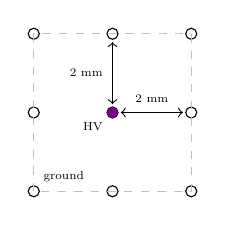
\begin{tikzpicture}%[very thick]
    \tikzset{
        every node/.style={font=\scriptsize}
    }
    
    \foreach \i in {0, 1, 2} {
        \foreach \j in {0, 1, 2} {
            \draw (\i,\j) circle [radius=2pt];
            \coordinate (A\i\j) at (\i,\j);
        }
    }

    \fill [violet] (1,1) circle [radius=2pt];
    \draw [dashed, gray!50] (0,0) rectangle (2,2);

    \draw [<->, shorten <=3pt, shorten >=3pt] (A11) -- (A21) node[midway, above] {\scalebox{0.6}{2 mm}};
    \draw [<->, shorten <=3pt, shorten >=3pt] (A11) -- (A12) node[midway, left] {\scalebox{0.6}{2 mm}};
    \node [below left] at (A11) {\scalebox{0.6}{HV}};
    \node [above right] at (A00) {\scalebox{0.6}{ground}};


\end{tikzpicture}


\end{document}